Shadows are the result of an surface being occluded from a direct light source by another object in the scene. To determine whether this is the case, we can define a shadow ray $S$ as follows:
$$S = \Vec{P} - t\hat{L}_n$$
Where $\Vec{P}$ is a point of intersection on a scene object and $\hat{L}_n$ is the direction of light source $n$. Note that $t\hat{L}_n$ is being subtracted from the ray's origin as the shadow ray should point towards the light source from the point of intersection.
\begin{figure}[H]
    \centering
    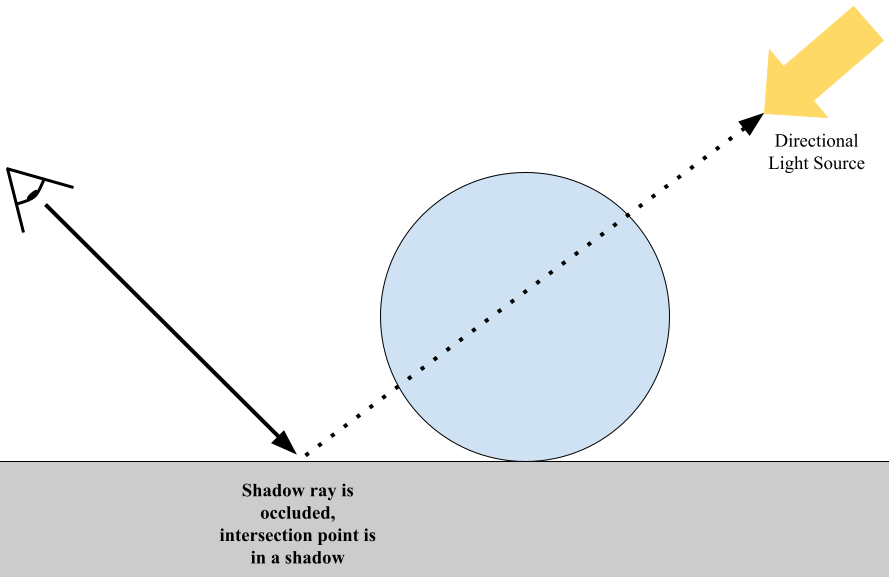
\includegraphics[scale=0.4]{figures/Shadows.png}
    \caption{Diagram of shadow rays}
    \label{fig:shadow_diag}
\end{figure}
\noindent
To determine whether the intersection point is in a shadow or not, we must simply cast the shadow ray into the scene and check for intersections with other scene objects. If an intersection is found, then the intersection point is in a shadow and should only receive ambient lighting. If not, then the intersection point is illuminated by a light source and should receive both ambient and diffuse lighting components. Implementing this logic gives us the following image when adding another, much larger sphere with a different color underneath our original.
\begin{figure}[H]
    \centering
    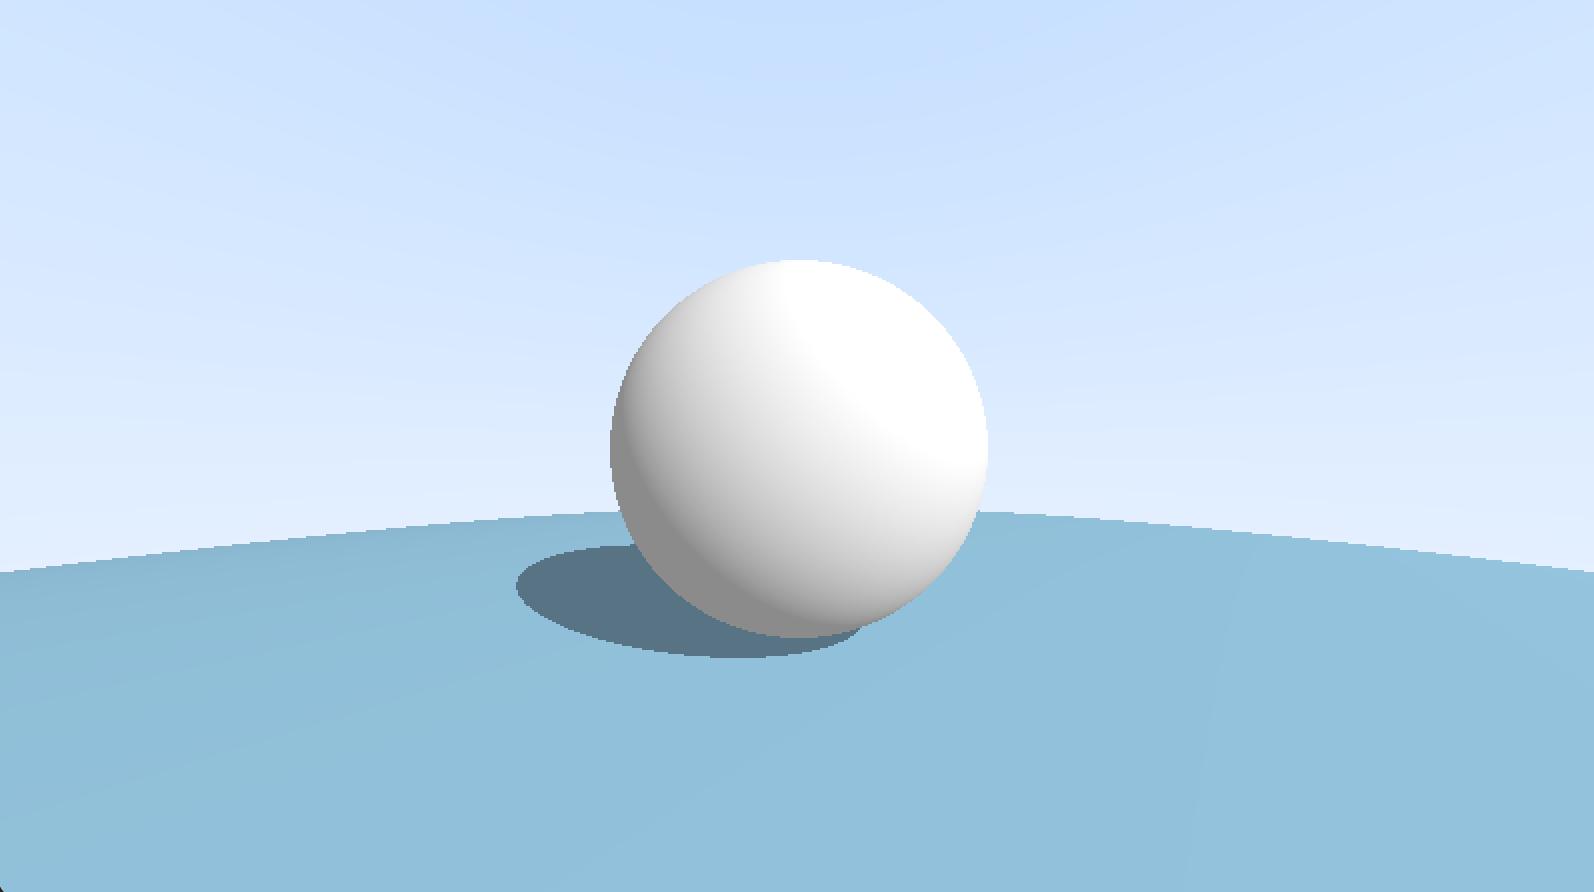
\includegraphics[scale=0.5]{figures/SphereShadows.png}
    \caption{A scene with two spheres to demonstrate shadows}
    \label{fig:sphere_shadows}
\end{figure}
\noindent
You may notice that the shadow illustrated in the image above ends abruptly, unlike shadows in the real world which are much softer. This is because points on the surfaces of objects can be partly occluded from light sources, creating a \textit{penumbra}, or soft shadow, which is not accounted for in this implementation. However, this effect can be achieved in a ray tracer by casting many shadow rays, each with slight randomness added to their direction, and averaging whether they are occluded or not, adjusting the strength of the shadow accordingly.